\subsection{Class Diagram}
We have mostly, directly used the UI classes provided by QT directly but made minor changes wherever neccessary. \\
The new classes made are: \\

\begin{minipage}{\linewidth}
\centering
\captionof{table}{New Classes}
\begin{tabular}{|p{5cm}|p{5cm}|}
\hline
 ui::MainWindow & Class representing the main UI \\ \hline
 MyTextEdit & Represents the textarea used for showing and editing specRTL file content, extented from QTextEdit to include keyboard event. \cite{3} \\ \hline
 util & Namespace for utility classes and functions. \\ \hline
 util::getDriver(int aArgNum, char** aArgs) & Global function, entry point into parser. \\ \hline
 util::ThreadedParser & Threaded class to invoke parser multiple times. \\ \hline
 util::NodeMap & This constructs a map of nodes displayable on the UI. \\ \hline
 BNode & This is a wrapper on the node class, storing extra information related to UI. \\ \hline
 ListViewModel & It is the model for the list of patterns shown on the UI for wasy navigation. \\ \hline
 PatternDTO & Simple data transfer object class used as a container for Pattern information. \\ \hline
 MyGraphicsScene & Derived from QGraphicsScene to support mouse double click event. \\ \hline
\end{tabular}
\end{minipage}

\vspace{1cm}

\begin{minipage}{\linewidth}
\centering
\captionof{table}{New header files (interfaces)}
\begin{tabular}{|p{5cm}|p{5cm}|}
\hline
 mainwindow.h & Class declaration of the main UI class \\ \hline
 listviewmodel.h & Declaration for ListViewModel class \\ \hline
 bnode.h & Declaration for BNode class \\ \hline
 util.h & New namespace util and declaration of getDriver(), NodeMap and ThreadedParser \\ \hline
 listviewmodel.h & Declaration of the model class for MyTextEdit. \\ \hline
 pattern\_dto.h & Declaration class for PatternDTO explained in above table. \\ \hline
 mygraphicsscene.h & Declaration for MyGraphicsScene. \\ \hline
\end{tabular}
\end{minipage}

\vspace{1cm}

\begin{minipage}{\linewidth}
\centering
\captionof{figure}{High level class diagram of the project}
 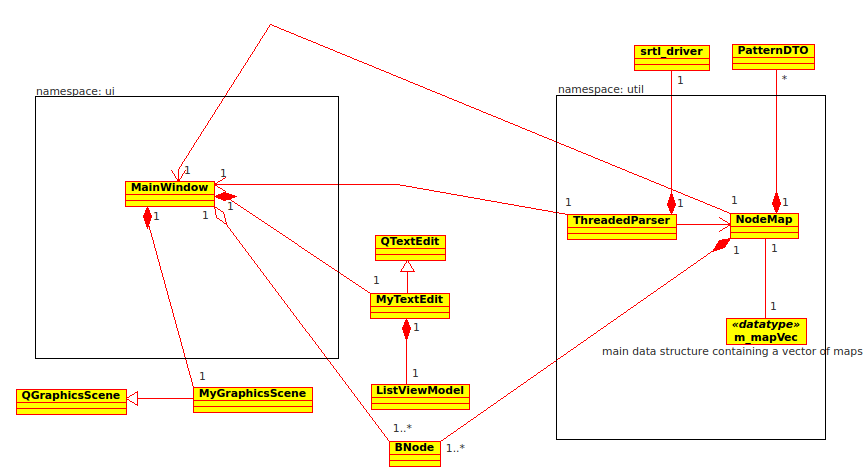
\includegraphics[scale=0.4]{classdiag} 
\end{minipage}